\documentclass[12pt,a4paper,openright,twoside]{book}
\usepackage[utf8]{inputenc}
\usepackage{disi-thesis}
\usepackage{code-lstlistings}
\usepackage{notes}
\usepackage{shortcuts}
\usepackage{acronym}

\school{\unibo}
\programme{Corso di Laurea Magistrale in Ingegneria e Scienze Informatiche}
\title{Fancy Title}
\author{Alberto Donati}
\date{\today}
\subject{Supervisor's course name}
\supervisor{Prof. Supervisor Here}
\cosupervisor{Dott. CoSupervisor 1}
\morecosupervisor{Dott. CoSupervisor 2}
\session{IV}
\academicyear{2022-2023}

% Definition of acronyms
\acrodef{IoT}{Internet of Thing}
\acrodef{vm}[VM]{Virtual Machine}


\mainlinespacing{1.241} % line spacing in mainmatter, comment to default (1)

\begin{document}

\frontmatter\frontispiece

\begin{abstract}
    Considering that companies have an increasing number of server connected to the network, IT professionals increasingly find themselves with machines on which to perform the same tasks.
    Therefore, systems that could automate tasks on large numbers of machines in parallel have been created and are increasingly being used.
    This thesis aims to compare and evaluate different server automation and orchestration systems, analyzing their features, advantages, and disadvantages.
    It will then go on to provide a summary overview of the reasons why professionals choose one alternative over another.
\end{abstract}

%\begin{dedication} % this is optional
%Optional. Max a few lines.
%\end{dedication}

%\begin{acknowledgements} % this is optional
%Optional. Max 1 page.
%\end{acknowledgements}

%----------------------------------------------------------------------------------------
\tableofcontents   
\listoffigures     % (optional) comment if empty
\lstlistoflistings % (optional) comment if empty
%----------------------------------------------------------------------------------------

\mainmatter

%----------------------------------------------------------------------------------------
\chapter{Introduction}
\label{chap:introduction}
%----------------------------------------------------------------------------------------

This thesis aims to compare and evaluate different server automation and orchestration systems.
It will provide also a summary overview, useful for professionals of IT to compare solutions.

\paragraph{Structure of the Thesis}

\note{At the end, describe the structure of the paper}

\chapter{State of the art}

\section{What are automation systems}
Automation systems are software tools that allow you to manage, monitor, and automate operations on a large number of servers. These systems can include features such as automatic provisioning, configuration management, service orchestration, performance monitoring, and troubleshooting.
An example of these systems is \textbf{Ansible}, which uses an agentless management model to connect to servers and perform automation tasks. Other examples include Puppet, Chef, and SaltStack, which offer similar features but use different approaches for server management.
These automation systems can be particularly useful in environments with a large number of servers, where manual management of each server would be inefficient and prone to errors. Through automation, organizations can improve operational efficiency, reduce errors, and free up IT staff to focus on other works.
Automation systems aims to simplify the execution of repetitive task.

\section{Who uses automation systems}

\section{When it makes sense (or doesn't make sense) to automate operations}

\section{What are the main systems}

\section{OpenSource and Closed Source, when OpenSource becomes Closed for some use cases}

%I suggest referencing stuff as follows: \cref{fig:random-image} or \Cref{fig:random-image}

%\begin{figure}
%    \centering
%    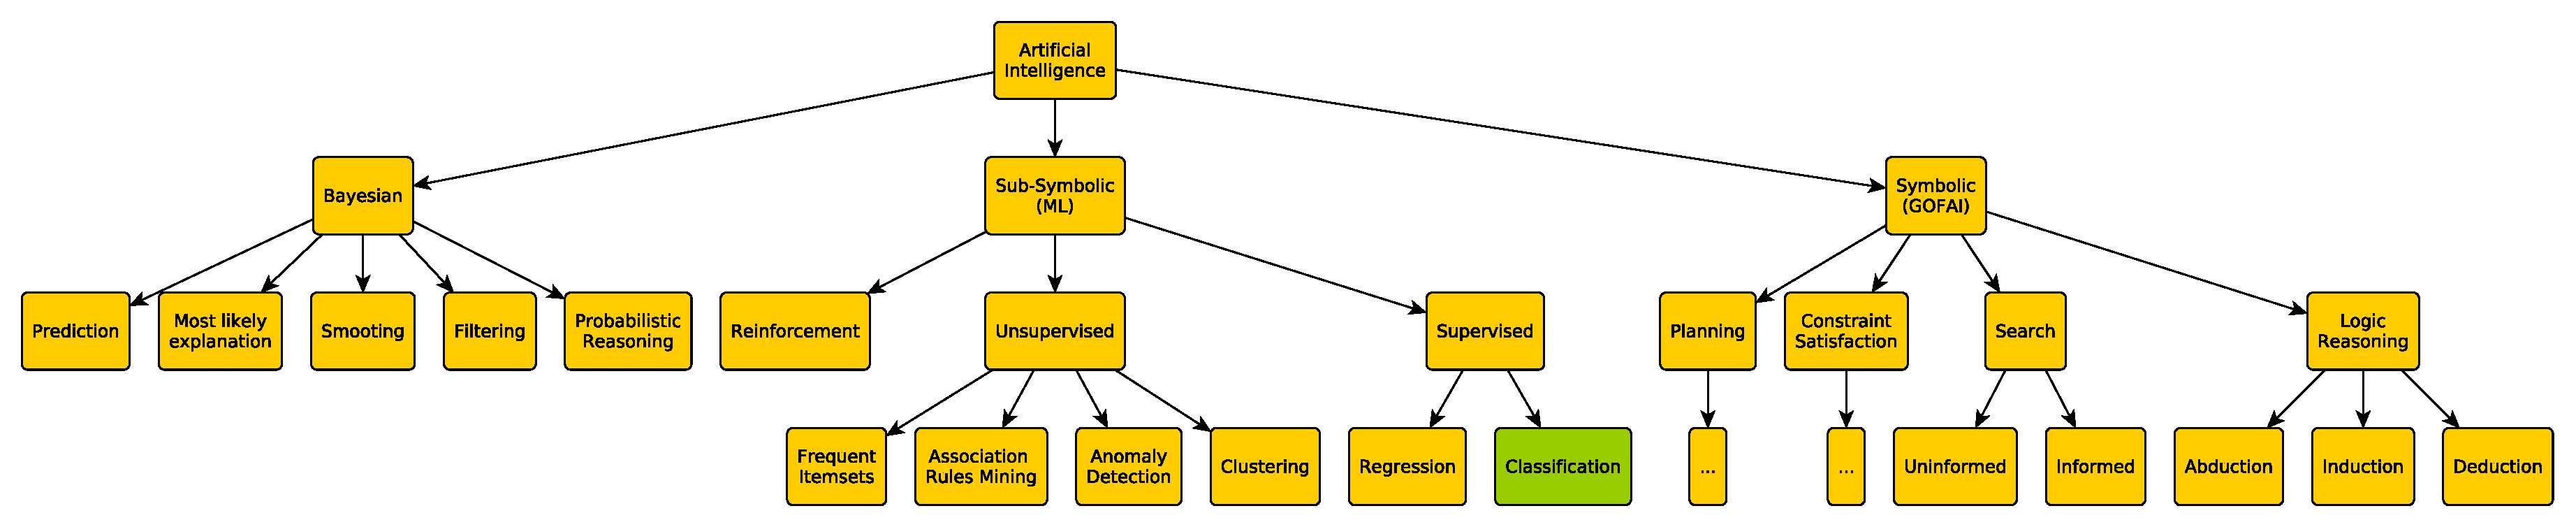
\includegraphics[width=.8\linewidth]{figures/random-image.pdf}
%    \caption{Some random image}
%    \label{fig:random-image}
%\end{figure}

\chapter{Ansible}

\section{The begin of Ansible}

Michael DeHaan define Ansible:
"Ansible is a configuration management tool, deployment tool, and ad-hoc task execution tool all in one."

The observation that formed the basis of Michael DeHaan's idea was that several online stores used separate tools for configuration, deployment, and yet another for task execution. This was because there was not one technology that could perform all these functions.
He also wanted Ansible to be as extensible as possible, that is, modules could be written in any language that could return JSON or key-value pairs.

One of the basic concepts that Micheal specified from the beginning was that configuration should be extremely simple, so without using configuration files, daemons and databases. Ansible from the beginning used a file with the machines that were to be managed written on it. Only the machines described in that file were managed, in case they were not included they would not be managed.

Quoting Micheal on his motivations for creating Ansible:
"While part of starting Ansible was to show the world there was an easier way -- to take those lessons from Red Hat, the field, and a long history of building systems management applications -- it was mostly to build the tool that (A) I actually wanted to use, and (B) was a tool that you could not use for six months, come back to, and still remember. I couldn't bring myself to be settled with the tools we had to use, it was too frustrating. As a developer myself, I wanted to write development code, I didn't want to spend 50\% of my time fighting with the automation tooling and have the automation itself be a source of frustration. I wanted to help all of these IT environments I was finding myself in, and also help myself as a consumer of those environments."

The motivation of Micheal about the project was:
"As a software developer, I myself can emphasize -- the software design/development/testing process is frequently painful, and I would rather think of infrastructure as being data-driven. Data is supposed to be simple, programs are often not. This is why I made Ansible."

\subsection{History}
In 2006 Michael DeHaan was working at Red Hat's Emerging Technologies group, a research unit under Red Hat. Emerging Tech was created specifically where people could could work on virtually anything they thought people needed.

Still those years, RedHat was very interested in configuration management. An early prototype of application virtualization management used Cobbler for provisioning the base operating system and Puppet for configuring virtual machines.

This project did not take off and Michael DeHaan attributed the cause to the fact that it was complex to write the detail under virtual applications, but Red Hat virtualization was also still in its early days.

Greg DeKoenigsberg was a Fedora community character and created a group with Michael DeHaan, Adrian Likins and Seth Vidal (author of yum). They wanted to create another very democratic open-source project in Red Hat, one that could have a wide variety of contributors and solve new problems. They thought back to busrpc. This project existed because it filled the gaps between Cobbler and Puppet. Cobbler could provide a system, and Puppet could put in configuration files, but because Puppet was too declarative you couldn't use it to do things like restart servers or do all the "ad hoc" tasks. In the past, Red Hat was exploring CIM, but there were not many good implementations of API support for Linux, so it would not be possible to build an open source project that would be able to rescout community success around CIM. The idea that was followed was to create an API-like channel for managing applications to configure systems, This idea was called Func.

Func was based on a central server reaching out to a remote node to send automation orders. It was called the central server "overlord" and each of the remote machines "minions." 

Other clones of Func were also created. Fabric and Capistrano also existed, but the team od Func wanted something more of an API and less of a script. Func was later used by Tumblr, and Steve Salesvan, who was interning at Red Hat at the time, continued to maintain it for Tumblr.

Michael therefore wanted to build a configuration management system on top of Func, tentatively called "Remote Rocket Surgery."

Cobbler, Puppet and Func formed some of the earliest DevOps-friendly automation tools, with Cobbler sometimes doing the provisioning and Func being used to launch Puppet.

After leaving RedHat and a brief term at Puppet, Micheal saw that the language often divided potential users and that the most important thing in automation tools, simplicity, should be a priority.

So Ansible began as a project in the beginning of 2012. It took off quickly due to many sysadmins and developers knowing Micheal.
Also, people from Fedora Infrastructure, replaced their Puppet automation with Ansible and so Fedora help Ansible to grow and also used as a test platform.

Like Func, it persues a "batteries included" philosophy, allowing everyone to contribute to the main modules and forming an active community of users.

After a period when Micheal was working on automation of OpenStack with Puppet, the project started to take off on GitHub, and soon the company was founded.

Ansible increase and Micheal and others had a good-sized company supporting it and more importantly building great products on top of it.

On 2015 Ansible was acquired from RedHat\cite{ansibleRedHat}.

Now, Ansible is currently one of the most used automation tool.

\section{Purpose of the technology}
Ansible is a technology used for automation. It allows from any environment to manage the automation of commands on other machines.
The files used for the description and therefore the execution of the scripts are called Playbooks.
Ansible is based on the Python language, so it is cross-platform.
Usually, its use is recommended in a Linux environment, some features are slightly different on a Windows environment.
Considering that most servers have a Linux kernel, the tests will focus on a Linux environment.
Ansible is ideal for managing IT environments, as it can automate tasks on a multitude of nodes simultaneously.

\subsection{Best points of Ansible}
\begin{itemize}
    \item \textbf{Simple}: As syntax, the files are described in YAML language. YAML is easy to understand by those who have minimal knowledge of programming languages and is often used for configurations. In addition, most configuration management software is characterized by an agent and a server from which to start the orchestration. In this case, Ansible's agentless management makes it easy to manage machines.
    \item \textbf{Fast}: Ansible, in addition to having a low learning curve, has a fast configuration, not having agents that must be constantly active on the host machines. Ansible connects directly to the host machines via ssh, and it is enough to have Python installed on the host machines.
    \item \textbf{Efficient}: Considering that Ansible do not have active agents, this does not consume extra resources in the hosts where the automatisms are executed. Ansible take space and resources only during the execution of the activity on the controlled node.
    \item \textbf{Secure}: Considering that the connection from manager to controlled node is via ssh, no extra open ports are required.
\end{itemize}

\section{How the tool is shown to the community}

\section{Who supports and maintains the project}
\subsection{Statistics [Examples]}
            \subsubsection{Number of GitHub issues}
            \subsubsection{Issues that have been resolved}
            \subsubsection{How active is the community}
            \subsubsection{Management of user feedback}
            \subsubsection{Community repository for uploading projects}

\section{Main Ansible components}

\subsection{Inventory}
            The inventory defines the nodes (also called hosts) of the infrastructure on which Ansible performs automations.
            Even if you can pass the host names from the terminal, it is good practice to create the inventory file.
            The hosts are inserted into groups, so that you can run automations on multiple hosts at the same time.
            According to the Ansible documentation on inventory management\cite{ansibleDocInventory}, you can group the machines according to the following criteria:
            
            \begin{itemize}
                \item \textbf{What:} What purpose they were created for
                \item \textbf{Where:} Where the machines are located
                \item \textbf{When:} The stage of development they are assigned to
            \end{itemize}
            
            In addition, you can also make parent-child relationships, in which each machine inserted in a child group is also part of the parent group. All that can be done usingt the \texttt{children} attribute.
            Another function that might be useful, considering the inventories, are the variables, which can be defined for the groups (and also subgroups), through the \texttt{vars} attribute.

\subsubsection{Example Inventory Ansible}

\lstinputlisting[label={lst:exampleInventoryAnsible}]{listings/exampleInventoryAnsible.yaml}

\subsection{Modules}
Modules are small programs, which are called by tasks to perform operations on machines.
There are modules for different jobs we want to perform, some already provided by default, can be used from package installation to DevOps workflows.
One example is package installation via apt (ansible.builtin.apt).
There are also many modules provided by the community. If the community and default modules are not enough, there is the option of creating custom modules\cite{ansibleDocNewModules}.
Ansible modules are designed to be idempotent, which means that they will make changes to managed nodes only when necessary. This ensures that managed nodes remain in the desired state, even if the playbook is run multiple times.

\subsection{Play}
The play contains the list of tasks to be executed (at least one). The play also contains the list of hosts on which the tasks will be executed; it may contain variables and other commands.
Plays within the playbook are executed from top to bottom. Considering that playbooks are written in YAML, they are easily readable.

\subsection{Task}
The Task is the action we need to execute towards the controlled machine. The commands will be executed by calling the choosen modules with various parameters.

\subsection{Playbook}
Playbook is a collection of one or more Plays.
These are sorts of books that contain different Plays, which depending on the request, will go to be executed. Playbooks use basic programming constructs such as loops and conditionals, which allows for greater flexibility in controlling the code.
Playbooks can be reused, so you can create the best combination according to your scenario.

\subsubsection{Example Playbook Ansible}

\lstinputlisting[label={lst:examplePlaybookAnsible}]{listings/examplePlaybookAnsible.yaml}

In this example, the names of Plays are \texttt{Package installation} and \texttt{Package uninstallation}.

The execution will be target to the host group \texttt{campusNord}, with superuser privileges, given by the attribute-value \texttt{become : yes}.

In addition, \texttt{vars} defines two variables: \texttt{package\_name\_1} and \texttt{package\_name\_2}, which represent the names of the packages to install.

The Tasks called \texttt{Install package 1} and \texttt{Install package 2} install the packages specified by the variables \texttt{package\_name\_1} e \texttt{package\_name\_2}.

Considering that Ansible is idempotent,
in case the packages were already installed in the system, Ansible will not perform any operation and will not reinstall them either. If instead the packages were not already present in the system, Ansible, through the apt module, will install them.

In the Task \texttt{Uninstall MongoDB}, the apt module takes as input directly the value \texttt{mongodb}, and sets the state to \texttt{absent} to make sure that, if present, it is removed.

%commento
%paragraph{Roles}

%Roles: i roles (ruoli) sono dei componenti dei playbook che raggruppano operazioni legate tra di loro con uno scopo specifico. Queste vengono di solito unificate per avere più riusabilità delle stesse. Se il ruolo definito è processo standard, è facile che qualcuno lo abbia già implementato e lo si può scaricare da Ansible Galaxy!.

%differenzeeee plugin e modules
%https://docs.ansible.com/ansible/latest/dev_guide/developing_locally.html#developing-locally

\section{Characteristics}

\subsection{Platforms available (Linux,Windows,MacOS)}
\subsection{Operating Systems supported and recommended}
\subsection{Language of the project}
\subsection{Language for automation definition}
\subsection{Architecture, agent or agentless}
\subsection{Structure of the project}
\subsubsection{Deep structure of of the project (how it is the open source internal project)}
\subsection{Documentation of the project}
\subsection{Extensions of the project (modules, libraries)}

\section{Installation and configuration}


As indicated in the official documentation\cite{ansibleDocInstall}:

Ansible community packages are distributed in two ways:

- \textbf{ansible-core} a minimalist language and runtime package that contains a set of Ansible.Builtin.

- \textbf{ansible} a much larger package "with batteries included" that adds a curated selection from the Ansible Collections community to automate a wide range of devices.

The official method involves pip and then installing Ansible via pip.

\lstlisting[label={lst:installAnsibleViaPip}]
{
sudo apt install python3-pip
}

%\texttt{pip} occupa circa 250 MegaByte di spazio,

%Poi con pip per installare Ansible (core):
%\begin{listing}[H]
%\begin{minted}{BASH}
%python3 -m pip install --user ansible-core
%\end{minted}
%\end{listing}

%Su ubuntu.04 LTS,
%Considering that Python3 in pre installed in Ubuntu, it is possible to install Ansible via \texttt{apt}

%\begin{listing}[H]
%\begin{minted}{BASH}
%sudo apt install ansible-core
%\end{minted}
%\end{listing}

%L'installazione richiede solamente circa 80 MegaByte,

%prova questo
%https://riptutorial.com/ansible/example/5069/hello--world







\chapter{Conclusion}
Scrivere la conclusione

\subsection{Comparations}
Esempio comparazione tecnologie

\subsection{Consideration}
Considerazioni finali


%\section{Some cool topic}

\chapter{Contribution}

%You may also put some code snippet (which is NOT float by default), eg: \cref{lst:random-code}.

%\lstinputlisting[float,language=Java,label={lst:random-code}]{listings/HelloWorld.java}

%\section{Fancy formulas here}

%----------------------------------------------------------------------------------------
% BIBLIOGRAPHY
%----------------------------------------------------------------------------------------

\backmatter

\nocite{*} % comment this to only show the referenced entries from the .bib file

\bibliographystyle{alpha}
\bibliography{bibliography}

\end{document}